\documentclass[sigconf,nonacm]{acmart}

\AtBeginDocument{%
  \providecommand\BibTeX{{Bib\TeX}}}

\acmConference[Explainable and Trustworthy AI - Project]{}{}{}
\settopmatter{printacmref=false}
\renewcommand\footnotetextcopyrightpermission[1]{}
\pagestyle{plain}

\begin{document}

\title{Evaluating the Quality of Explanations under a Cognitive Feature Budget}

\author{Stefano Zizzi}
\affiliation{%
  \institution{Politecnico di Torino}
  \city{Turin}
  \country{Italy}
}

\author{Michelangelo Ungolo}
\affiliation{%
  \institution{Politecnico di Torino}
  \city{Turin}
  \country{Italy}
}

\author{Miriana Sette}
\affiliation{%
  \institution{Politecnico di Torino}
  \city{Turin}
  \country{Italy}
}

\begin{abstract}
Local explanation methods are often evaluated with complete explanations, while
users usually inspect only a few features. This project introduces
Complexity-Calibrated Local Concordance (CCC), a functionally-grounded metric
that tests whether an additive explanation remains faithful after top-$K$
truncation. We implement an evaluation framework for tabular classification
using two UCI datasets, two black-box models, and three explainers: LIME, SHAP,
and MAPLE. The experiments show that SHAP is the strongest method under compact
faithfulness, but also that exact full fidelity does not guarantee a
faithful compact explanation. CCC therefore complements existing XAI metrics by
making the trade-off between fidelity and human-sized explanations explicit.
\end{abstract}

\keywords{Explainable AI, local explanations, faithfulness, cognitive complexity}

\maketitle

\section{Introduction}
Explainable Artificial Intelligence (XAI) is used to make black-box predictions
inspectable by users, developers, and domain experts. In tabular classification,
local explanation methods such as LIME~\cite{ribeiro2016lime}, SHAP~\cite{lundberg2017shap},
and MAPLE~\cite{plumb2018maple} are particularly common because they express
each prediction as a set of feature contributions. The central evaluation
problem is whether those contributions are faithful to the model rather than
merely plausible to a human observer~\cite{doshi2017towards}.

The EQE project (Evaluating the Quality of Explanations) focuses on a specific
blind spot in this evaluation problem. Many faithfulness metrics evaluate the
complete explanation, but complete explanations can contain all available
features. A user-facing explanation, instead, should remain useful after being
reduced to a small number of high-impact features. This is not only a design
preference: Miller's classic work on working-memory limits suggests that humans
can actively process only a small number of information units at once~\cite{miller1956magical}.
For this reason, the project evaluates explanations under a feature budget
$K \in \{4,\ldots,9\}$.

The contribution is a benchmark and metric centered on \emph{compact
faithfulness}. We introduce Complexity-Calibrated Local Concordance (CCC), which
measures how well a top-$K$ truncated additive explanation reconstructs the
black-box probability. The project implements CCC together with standard
comparison metrics and applies it to LIME, SHAP, and MAPLE on the UCI Breast
Cancer Wisconsin Diagnostic and Adult datasets.

\section{Related Work}
XAI evaluation is usually divided into human, application, and functional
levels~\cite{doshi2017towards}.
Human-grounded evaluation studies whether people can use explanations in
simplified tasks; application-grounded evaluation studies utility in a real
domain workflow; and functionally-grounded evaluation uses computational proxies
when human studies are not available. This project belongs to the third
category: it evaluates formal properties of explanations produced for trained
classifiers.

\subsection{Local Explanation Methods}
LIME fits a sparse local surrogate around the instance to be explained
~\cite{ribeiro2016lime}. It is model-agnostic and intuitive, but its output can
depend strongly on perturbation sampling, feature scaling, and the local linear
fit. SHAP computes feature attributions based on Shapley values and satisfies
desirable axioms for additive explanations~\cite{lundberg2017shap}. In this
project SHAP is implemented through KernelExplainer, using a sampled training
background and the positive-class probability as the explained output. MAPLE
learns local linear explanations by combining random-forest neighborhoods with
supervised local regression~\cite{plumb2018maple}. In the codebase, MAPLE
coefficients are converted into per-instance additive contributions by
multiplying each coefficient by the corresponding feature value, so all three
explainers share the same interface: weights and intercepts.

\subsection{Evaluation Metrics}
The literature review conducted for the project identified several families of
functionally-grounded metrics. Fidelity metrics compare the explanation with the
black-box model. Sufficiency and comprehensiveness perturb relevant features to
check whether selected features preserve or remove prediction evidence.
Robustness metrics, including sensitivity and infidelity~\cite{yeh2019infidelity},
measure how explanations react to input perturbations. Benchmark projects such
as XAI-Bench~\cite{liu2021xaibench} and OpenXAI~\cite{agarwal2022openxai}
systematize these criteria across methods and datasets. Frameworks such as
LEAF~\cite{amparore2021leaf} also include local concordance and conciseness
criteria. However, these metrics usually treat faithfulness and compactness as
separate properties: one metric asks whether the full explanation is faithful,
another asks whether the explanation is small. CCC combines the two by asking
whether the explanation is still faithful \emph{after} enforcing a small
top-$K$ budget.

\section{Research Gap}
The project targets the gap between mathematical fidelity and usable fidelity.
For an additive explanation
$g(x)=w_0+\sum_i \phi_i(x)$, a method may be perfectly faithful when every
feature contribution is included. SHAP, for example, is designed to satisfy
local accuracy under the full additive reconstruction. But a practitioner may
show only the largest four to nine contributions in a dashboard, report, or
interactive tool. If the omitted contributions collectively matter, the compact
explanation can misrepresent the model even though the full explanation is
exact.

This gap is not captured by model accuracy either. A high-accuracy classifier
can be difficult to explain compactly, while a slightly less accurate model may
produce local attributions that concentrate prediction evidence in fewer
features. The research question is therefore:
\begin{quote}
  Given a black-box model and a local additive explainer, how much fidelity is
  preserved when only the top-$K$ feature contributions are shown?
\end{quote}
Answering this question helps compare explainers under a realistic cognitive
budget and provides a sanity check for feature rankings.

\section{Methodology}
\subsection{Complexity-Calibrated Local Concordance}
For each test instance $x$, the framework stores the black-box positive-class
probability $f(x)$, the explainer intercept $w_0$, and the additive
contribution vector $\phi(x)$. Let $S_K(x)$ be the indices of the $K$ largest
absolute contributions. The truncated local reconstruction is
\begin{equation}
  g_K(x) = w_0 + \sum_{i \in S_K(x)} \phi_i(x).
\end{equation}
Complexity-Calibrated Local Concordance is the mean squared error between the
black-box output and this truncated reconstruction:
\begin{equation}
  \mathrm{CCC}_K =
  \frac{1}{N}\sum_{j=1}^{N}\left(f(x^{(j)}) - g_K(x^{(j)})\right)^2.
\end{equation}
Lower CCC means that the explainer preserves local predictive fidelity using
only $K$ features.

The implementation intentionally does not multiply contributions by the raw
features during reconstruction: SHAP values are already additive
contributions, LIME returns local feature weights for the explained instance,
and MAPLE coefficients are converted into contributions inside the explainer
wrapper. This normalization is essential because CCC assumes a common additive
form across methods.

\subsection{Comparison Metrics}
Table~\ref{tab:metrics} summarizes the implemented metrics. Full MSE measures
the fidelity of the complete additive explanation. Random-$K$ MSE keeps $K$
random contributions from the same weight vector and is repeated 30 times; it
tests whether the explainer's top-$K$ ordering is better than arbitrary
selection. Sufficiency and comprehensiveness use a feature baseline, implemented
as the mean training vector, to evaluate prediction drift under input masking.
The current codebase also includes normalized CCC and top-$K$ degradation ratio
for cross-dataset comparison and truncation analysis.

\begin{table}[t]
  \caption{Metrics implemented in \texttt{core/metrics.py}.}
  \label{tab:metrics}
  \centering
  \small
  \begin{tabular}{p{0.27\columnwidth}p{0.47\columnwidth}p{0.14\columnwidth}}
    \toprule
    Metric & Quantity measured & Direction \\
    \midrule
    CCC & Top-$K$ reconstruction error & lower \\
    Full MSE & Full additive reconstruction error & lower \\
    Random-$K$ & Random top-$K$ baseline & lower \\
    Sufficiency & Drift when only top-$K$ inputs remain & lower \\
    Comprehensive. & Drift when top-$K$ inputs are removed & higher \\
    Normalized CCC & CCC divided by prediction variance & lower \\
    Degradation & CCC divided by full MSE & lower \\
    \bottomrule
  \end{tabular}
\end{table}

\section{Software Architecture}
The project is organized as a reproducible Python benchmark. The entry point
\texttt{core/main.py} reads \texttt{config.yml}, builds a matrix of
dataset--seed runs, executes them in parallel with joblib, and writes Markdown
results. The experiment orchestration is implemented in
\texttt{core/test\_framework.py}. For each dataset and seed, the orchestrator:
loads and scales the data, trains every configured model, generates
explanations for every model/explainer pair, caches the weights and intercepts,
and computes every metric for all configured values of $K$.

The data loaders support the local copies of the UCI Breast Cancer Wisconsin
Diagnostic and Adult datasets. Breast Cancer uses the WDBC files and recovers
descriptive feature names from metadata; Adult combines the train and test
files, removes missing values, one-hot encodes categorical attributes, and
standardizes features. The model wrappers expose a uniform \texttt{train},
\texttt{predict}, and \texttt{predict\_proba} interface for XGBoost~\cite{chen2016xgboost}
and a scikit-learn multilayer perceptron~\cite{scikit-learn}. The visualization
module generates summary charts from result files and per-instance top-$K$
reduction figures for presentation.

\section{Experimental Setup}
The main benchmark uses two public datasets: UCI Breast Cancer Wisconsin
Diagnostic~\cite{uciwdbc} and UCI Adult~\cite{uciadult}. The classifiers are
XGBoost and a neural network with two hidden layers of 100 units and a maximum
of 500 training iterations. The explainers are LIME, SHAP KernelExplainer, and
MAPLE. SHAP uses a sampled training background of size 100. MAPLE uses random
forest feature extraction, 100 estimators, a validation size of 100, a training
subsample of 2000 when available, and regularization 0.001. The benchmark
evaluates $K=4,5,6,7,8,9$ over seeds 42, 123, and 2026.

The results discussed below come from the 20260629 archive file under
\texttt{results/archive/}, which contains aggregate tables grouped by dataset,
model, explainer, and $K$. The run reports six dataset--seed executions and
includes model accuracy plus CCC, full MSE, sufficiency, comprehensiveness, and
random-$K$ MSE.

\begin{table}[t]
  \caption{Mean model accuracy across the three seeds.}
  \label{tab:accuracy}
  \centering
  \begin{tabular}{llr}
    \toprule
    Dataset & Model & Accuracy \\
    \midrule
    Adult & XGBoost & 0.874 \\
    Adult & Neural network & 0.821 \\
    Breast Cancer & XGBoost & 0.968 \\
    Breast Cancer & Neural network & 0.977 \\
    \bottomrule
  \end{tabular}
\end{table}

\begin{figure*}[t]
  \centering
  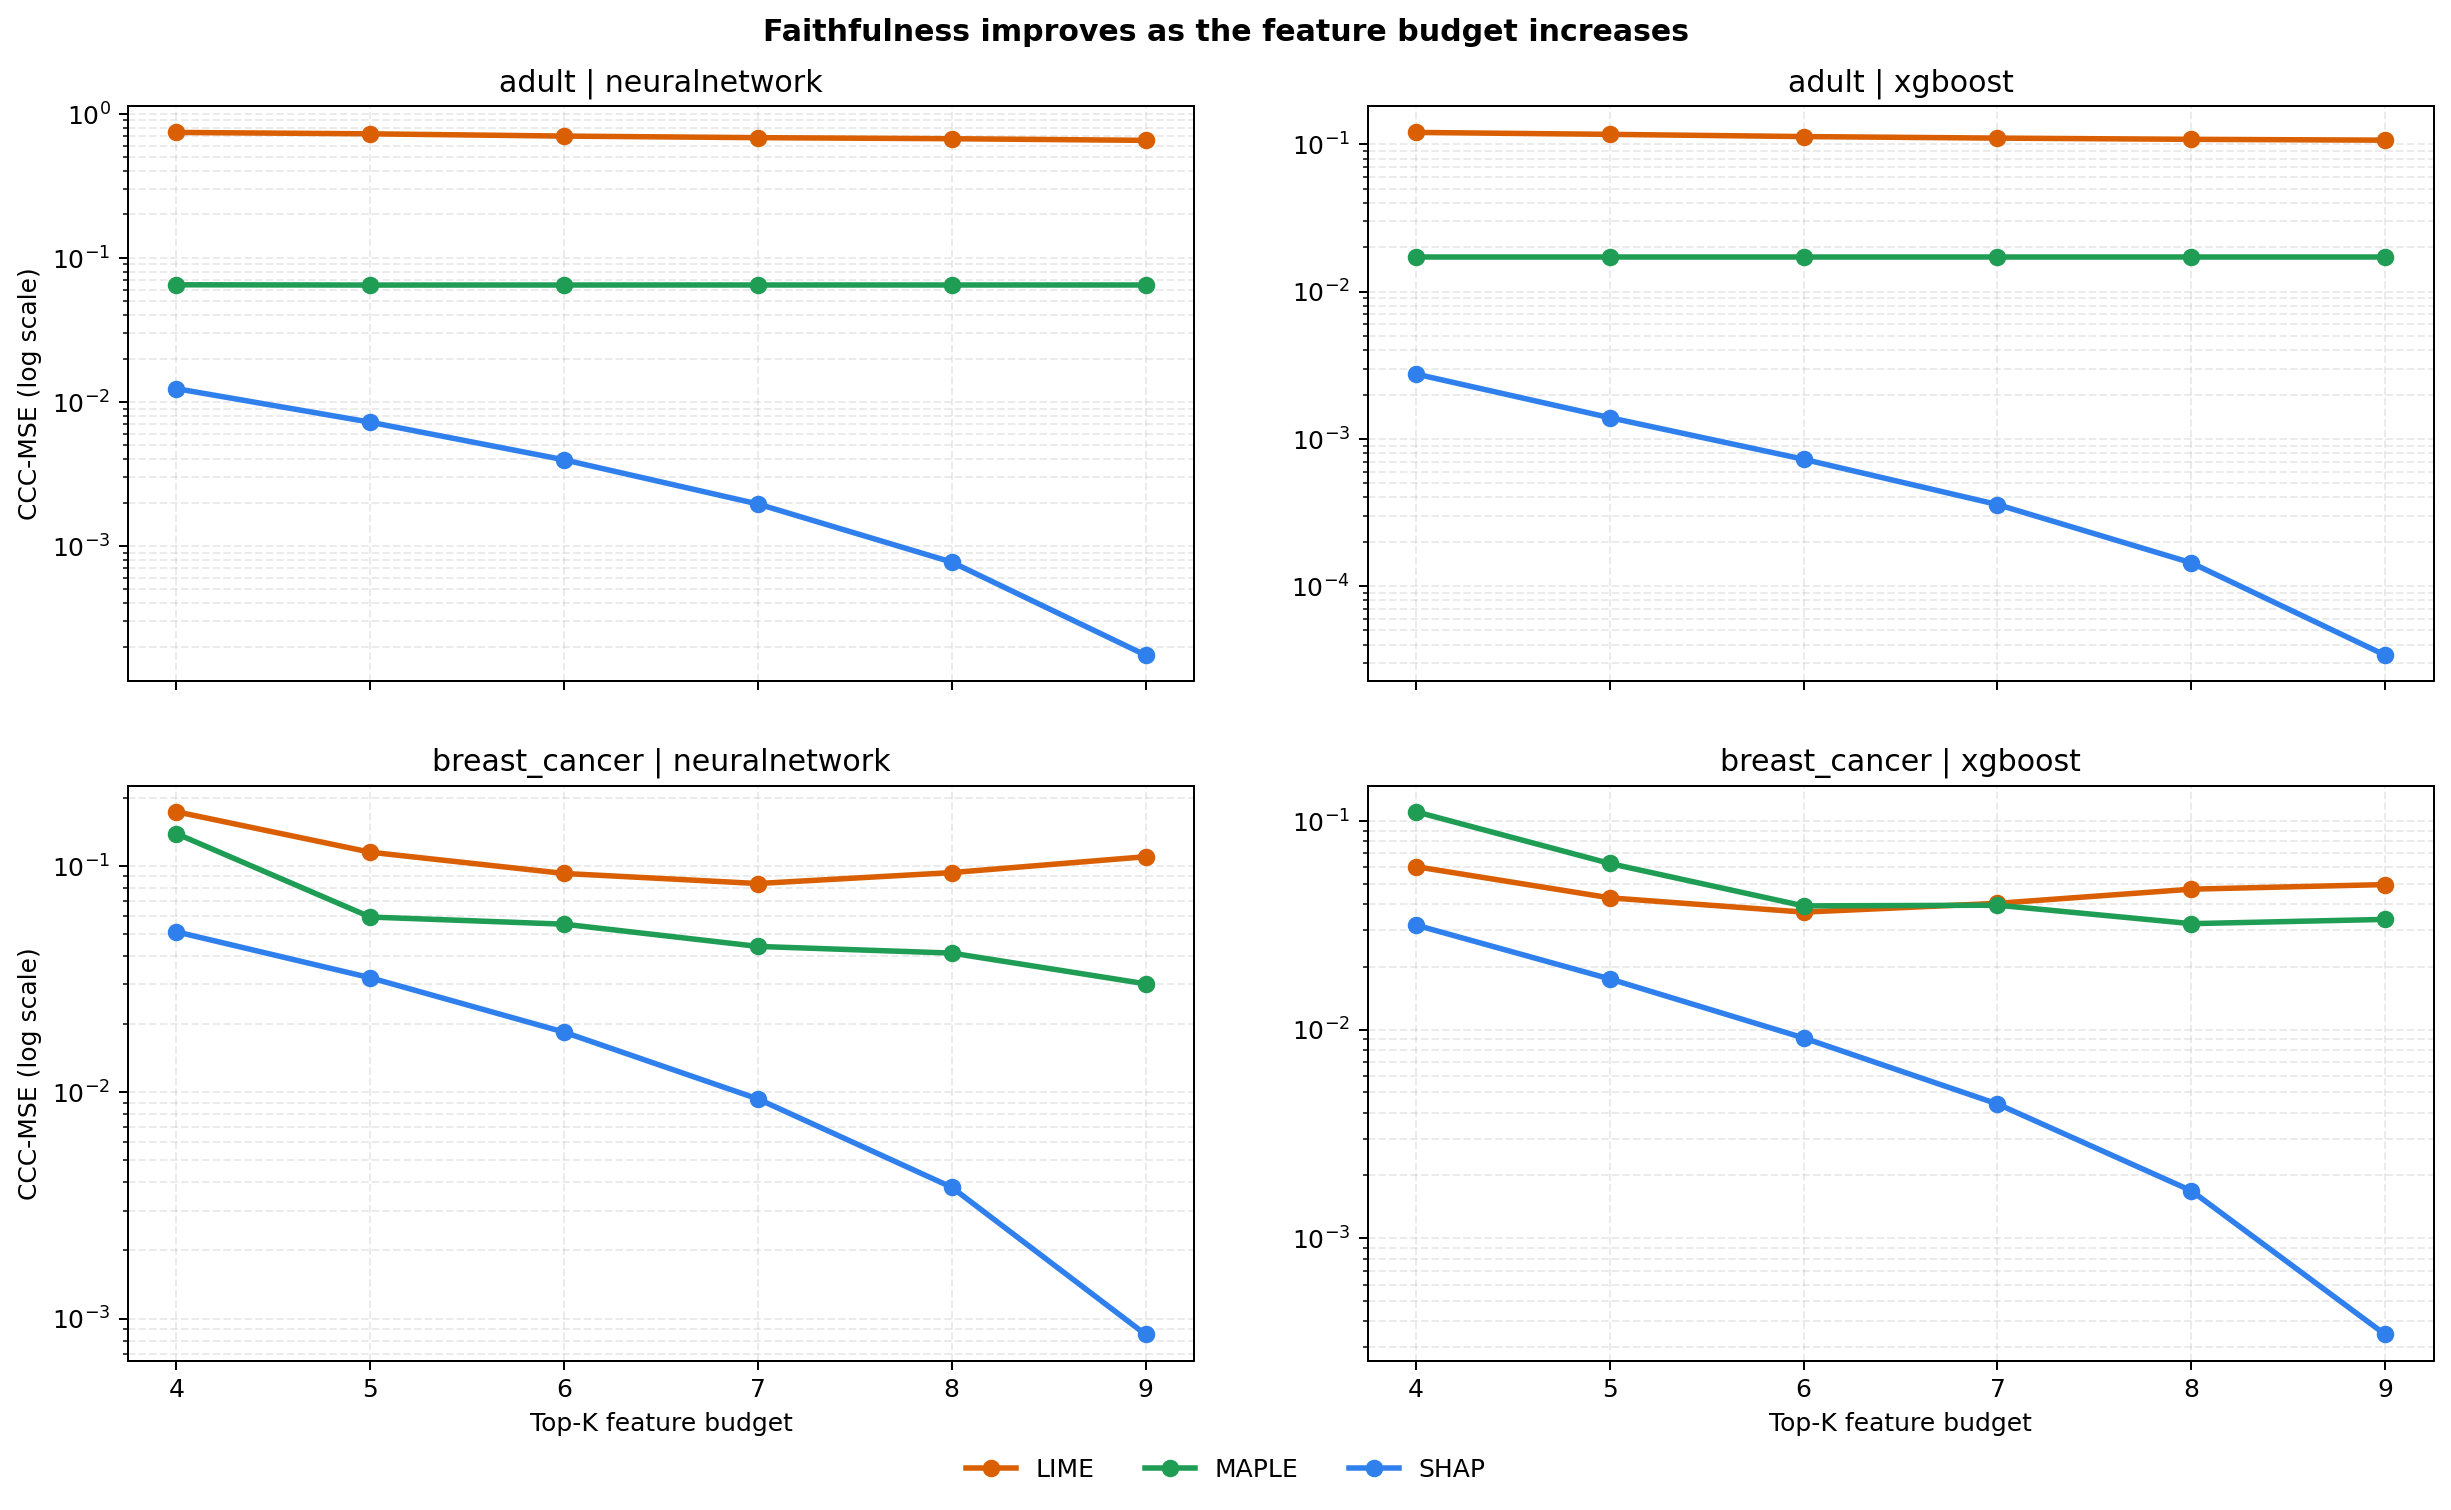
\includegraphics[width=0.95\textwidth]{../../../results/figures/presentation/ccc_mse_by_k.png}
  \caption{CCC as the feature budget increases. The figure was generated from
  the project visualization utilities. Lower curves indicate more faithful
  compact explanations.}
  \Description{Line plots of CCC MSE by K for each dataset and model, grouped by explainer.}
  \label{fig:ccc-by-k}
\end{figure*}

\begin{table*}[t]
  \caption{Representative aggregate CCC values from
  \texttt{results\_20260629\_105230.md}. Lower is better.}
  \label{tab:ccc-results}
  \centering
  \begin{tabular}{llrrrrrr}
    \toprule
    Dataset/model & Explainer & $K=4$ & $K=5$ & $K=6$ & $K=7$ & $K=8$ & $K=9$ \\
    \midrule
    Adult/NN & SHAP  & 0.0125 & 0.0074 & 0.0040 & 0.0020 & 0.0008 & 0.0002 \\
    Adult/NN & MAPLE & 0.0590 & 0.0590 & 0.0590 & 0.0590 & 0.0590 & 0.0590 \\
    Adult/NN & LIME  & 3.4195 & 3.3630 & 3.2186 & 3.0533 & 2.8499 & 2.6331 \\
    Adult/XGB & SHAP & 0.0029 & 0.0014 & 0.0007 & 0.0003 & 0.0001 & 0.0000 \\
    Adult/XGB & MAPLE & 0.0181 & 0.0180 & 0.0180 & 0.0179 & 0.0179 & 0.0179 \\
    Breast/XGB & SHAP & 0.0286 & 0.0160 & 0.0082 & 0.0037 & 0.0014 & 0.0003 \\
    Breast/XGB & MAPLE & 0.1210 & 0.0755 & 0.0556 & 0.0555 & 0.0405 & 0.0341 \\
    Breast/XGB & LIME & 0.0518 & 0.0396 & 0.0401 & 0.0408 & 0.0468 & 0.0530 \\
    \bottomrule
  \end{tabular}
\end{table*}

\section{Results and Analysis}
Model accuracy, shown in Table~\ref{tab:accuracy}, is not sufficient to select
an explainer. On Breast Cancer, the neural network is slightly more accurate
than XGBoost, but SHAP explanations for XGBoost reach lower compact error at
small and large $K$. On Adult, XGBoost is more accurate than the neural network,
but CCC still varies primarily with explainer choice rather than accuracy.

Figure~\ref{fig:ccc-by-k} and Table~\ref{tab:ccc-results} show three main
patterns. First, SHAP is the strongest method under CCC. Its error decreases
rapidly as $K$ increases, reaching near-zero values at $K=9$ on Adult/XGBoost
and Breast Cancer/XGBoost. This is expected from SHAP's additive local accuracy,
but the non-zero values at small $K$ are the important observation: a full SHAP
explanation can be exact while its compact version still loses fidelity.

Second, MAPLE is an intermediate baseline, with behavior that depends on the
dataset. On Breast Cancer/XGBoost, increasing $K$ reduces CCC from 0.1210 to
0.0341, meaning that the top-ranked contributions recover some predictive
signal. On Adult/NN and Adult/XGBoost, however, MAPLE is almost flat across
$K$. This suggests that the ranking does not concentrate the reconstruction
signal in a small subset of features, even if the full local approximation is
not terrible.

Third, LIME is unstable across settings. On Adult/NN, LIME CCC remains above
2.6 even at $K=9$, several orders of magnitude worse than SHAP. On
Breast Cancer/XGBoost, LIME is closer to SHAP for very small budgets but does
not improve monotonically with $K$: the error decreases until about $K=5$ or
$K=6$ and then rises again. This behavior indicates that adding more locally
weighted features does not necessarily make the truncated reconstruction closer
to the black-box probability.

\subsection{\texorpdfstring{Top-$K$ versus Random-$K$}{Top-K versus Random-K}}
The random-$K$ baseline gives CCC an internal sanity check. In most tested
settings, the explainer-selected top-$K$ features outperform random subsets of
the same explanation weights. For example, Adult/XGBoost SHAP at $K=9$ has CCC
around $3.1 \times 10^{-5}$, while random-$K$ MSE is about 0.086. Breast
Cancer/XGBoost SHAP at $K=9$ has CCC around 0.00027, while random-$K$ is about
0.113. This confirms that the top-ranked features preserve meaningful
prediction signal. When the gap is smaller, as for some MAPLE configurations,
the feature ranking is less informative.

\subsection{What CCC Reveals}
The main insight is that CCC separates three notions that can otherwise be
confused: model accuracy, full local fidelity, and compact local fidelity.
SHAP's full MSE is approximately zero because the full additive reconstruction
matches the explained model output, but CCC still exposes the cost of showing
only four or five features. MAPLE can have moderate full MSE but poor top-$K$
concentration. LIME can produce local weights whose selected features do not
reconstruct the probability well. These distinctions are directly relevant for
systems that display explanations to humans, because those systems normally
display only a subset of features.

\section{Limitations}
CCC applies naturally to additive explanations, but it is not directly suitable
for rule lists, counterfactual sets, prototypes, or explanations whose output is
not a decomposable sum. The metric also depends on the scale and calibration of
the model probability. For this reason the code includes normalized CCC, which
divides the error by the variance of black-box probabilities, although the main
archived run discussed here reports raw CCC. Perturbation metrics such as
sufficiency and comprehensiveness depend on the masking baseline; the current
implementation uses the mean training vector, which is simple and reproducible
but may create unrealistic inputs for correlated features. Finally, the
benchmark is limited to two datasets and two model families. The conclusions are
therefore strongest as evidence for the proposed evaluation protocol, not as a
universal ranking of all XAI methods.

\section{Reproducibility and Submission Material}
The implementation is contained in the submitted project archive and in the Git
repository \url{https://github.com/itsPinguiz/EQE}. The main entry point is
\texttt{core/main.py}; configuration is in \texttt{config.yml}; the archived
20260629 result file is under \texttt{results/archive/}; and the extended
technical notes are in \texttt{docs/relazione.md}. The public datasets are
referenced above and are also included locally under \texttt{datasets/}. Slides
are optional for submission; generated figures under \texttt{results/figures/}
can be reused for the final presentation.

\section{Future Work}
The most immediate extension is to broaden the benchmark without changing the
metric definition. Additional tabular datasets would test whether CCC remains
stable when the number of features, categorical sparsity, and class imbalance
change. Additional black-box models, such as calibrated linear models, random
forests, and gradient-boosted variants, would also clarify whether compact
faithfulness depends more on the explainer or on the geometry of the learned
decision function.

A second direction is to make the feature budget adaptive. The current report
uses fixed values from four to nine because they are easy to compare and align
with a cognitive-complexity motivation. In an interface, however, a useful
system could choose the smallest $K$ whose CCC falls below a model-specific
threshold, or expose a warning when no compact explanation reaches acceptable
fidelity. This would turn CCC from an offline benchmark metric into a runtime
quality-control signal for deployed explanation tools.

\section{Conclusions}
EQE contributes a compact-faithfulness evaluation of local explanations through
Complexity-Calibrated Local Concordance. CCC complements existing XAI metrics by
asking whether an additive explanation remains faithful after imposing a
human-sized feature budget. The benchmark shows that SHAP is the strongest
method under this criterion, MAPLE is a useful intermediate comparison, and
LIME is less reliable in the tested configurations. More importantly, the
results show that full-explanation fidelity and compact-explanation fidelity
are distinct evaluation targets. This makes CCC useful for practical XAI
settings where explanations must be both faithful to the model and short enough
to be inspected by a human.

\clearpage
\bibliographystyle{ACM-Reference-Format}
\bibliography{biblio}

\end{document}
\endinput
